\item A bola $C$ se desloca ao longo da ranhura de $A$ para $B$ com uma velocidade de \SI{.9}{\meter/\second} e uma aceleração de $\SI{.45}{\meter/\second^{2}}$, ambas medidas em relação à placa circular. Nesse mesmo instante, a placa gira com a velocidade angular e a aceleração angular mostradas. Determine a velocidade e a aceleração da bola nesse instante. 

\import{../answers/}{answer-13}

\vspace{-2cm}
\begin{flushleft}
	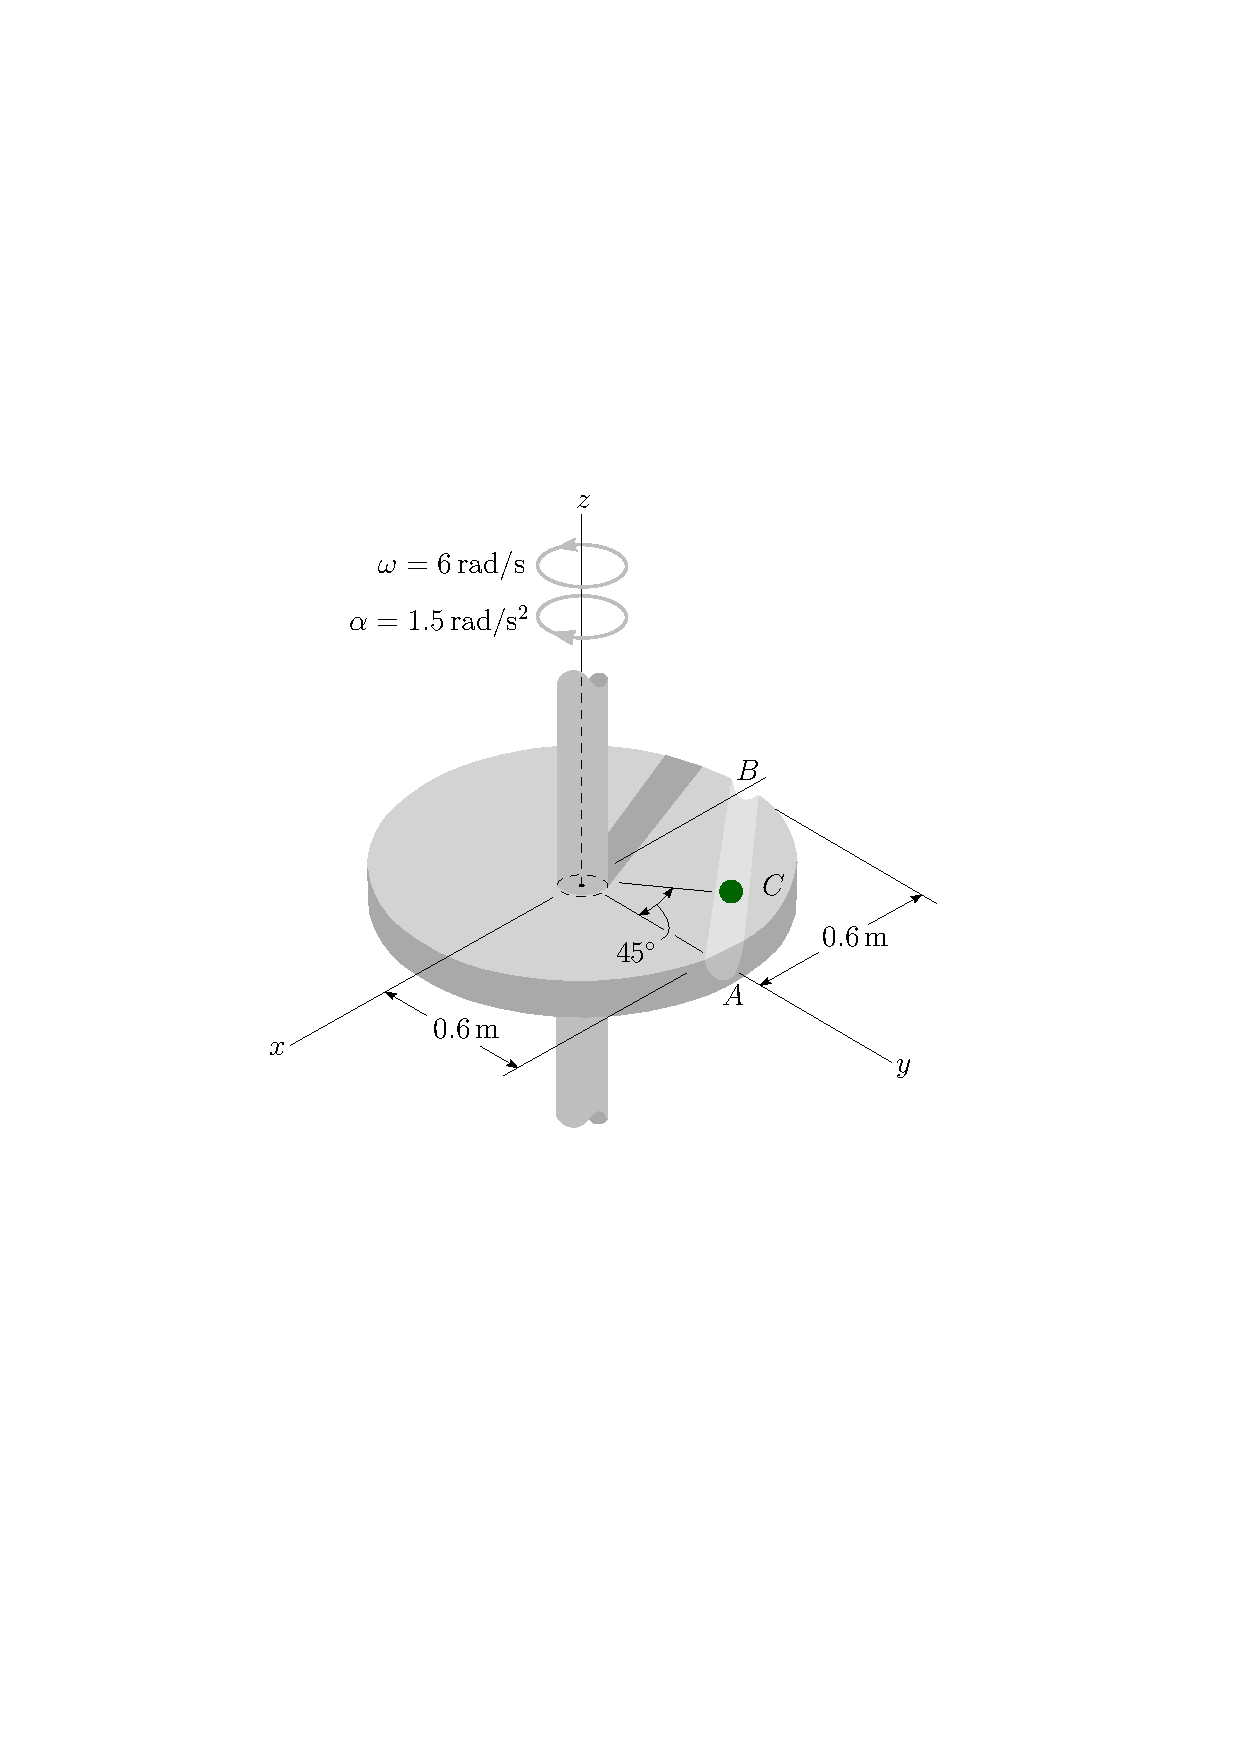
\includegraphics[scale=1]{images/draw_15}
\end{flushleft}